\documentclass[border=10pt]{standalone}

\usepackage{tikz}
\usepackage{tikzsymbols}
\usetikzlibrary{calc,patterns,shapes.geometric}

\def\centerarc[#1](#2)(#3:#4:#5){\draw[#1] ($(#2)+({#5*cos(#3)},{#5*sin(#3)})$) arc (#3:#4:#5);}

\begin{document}
	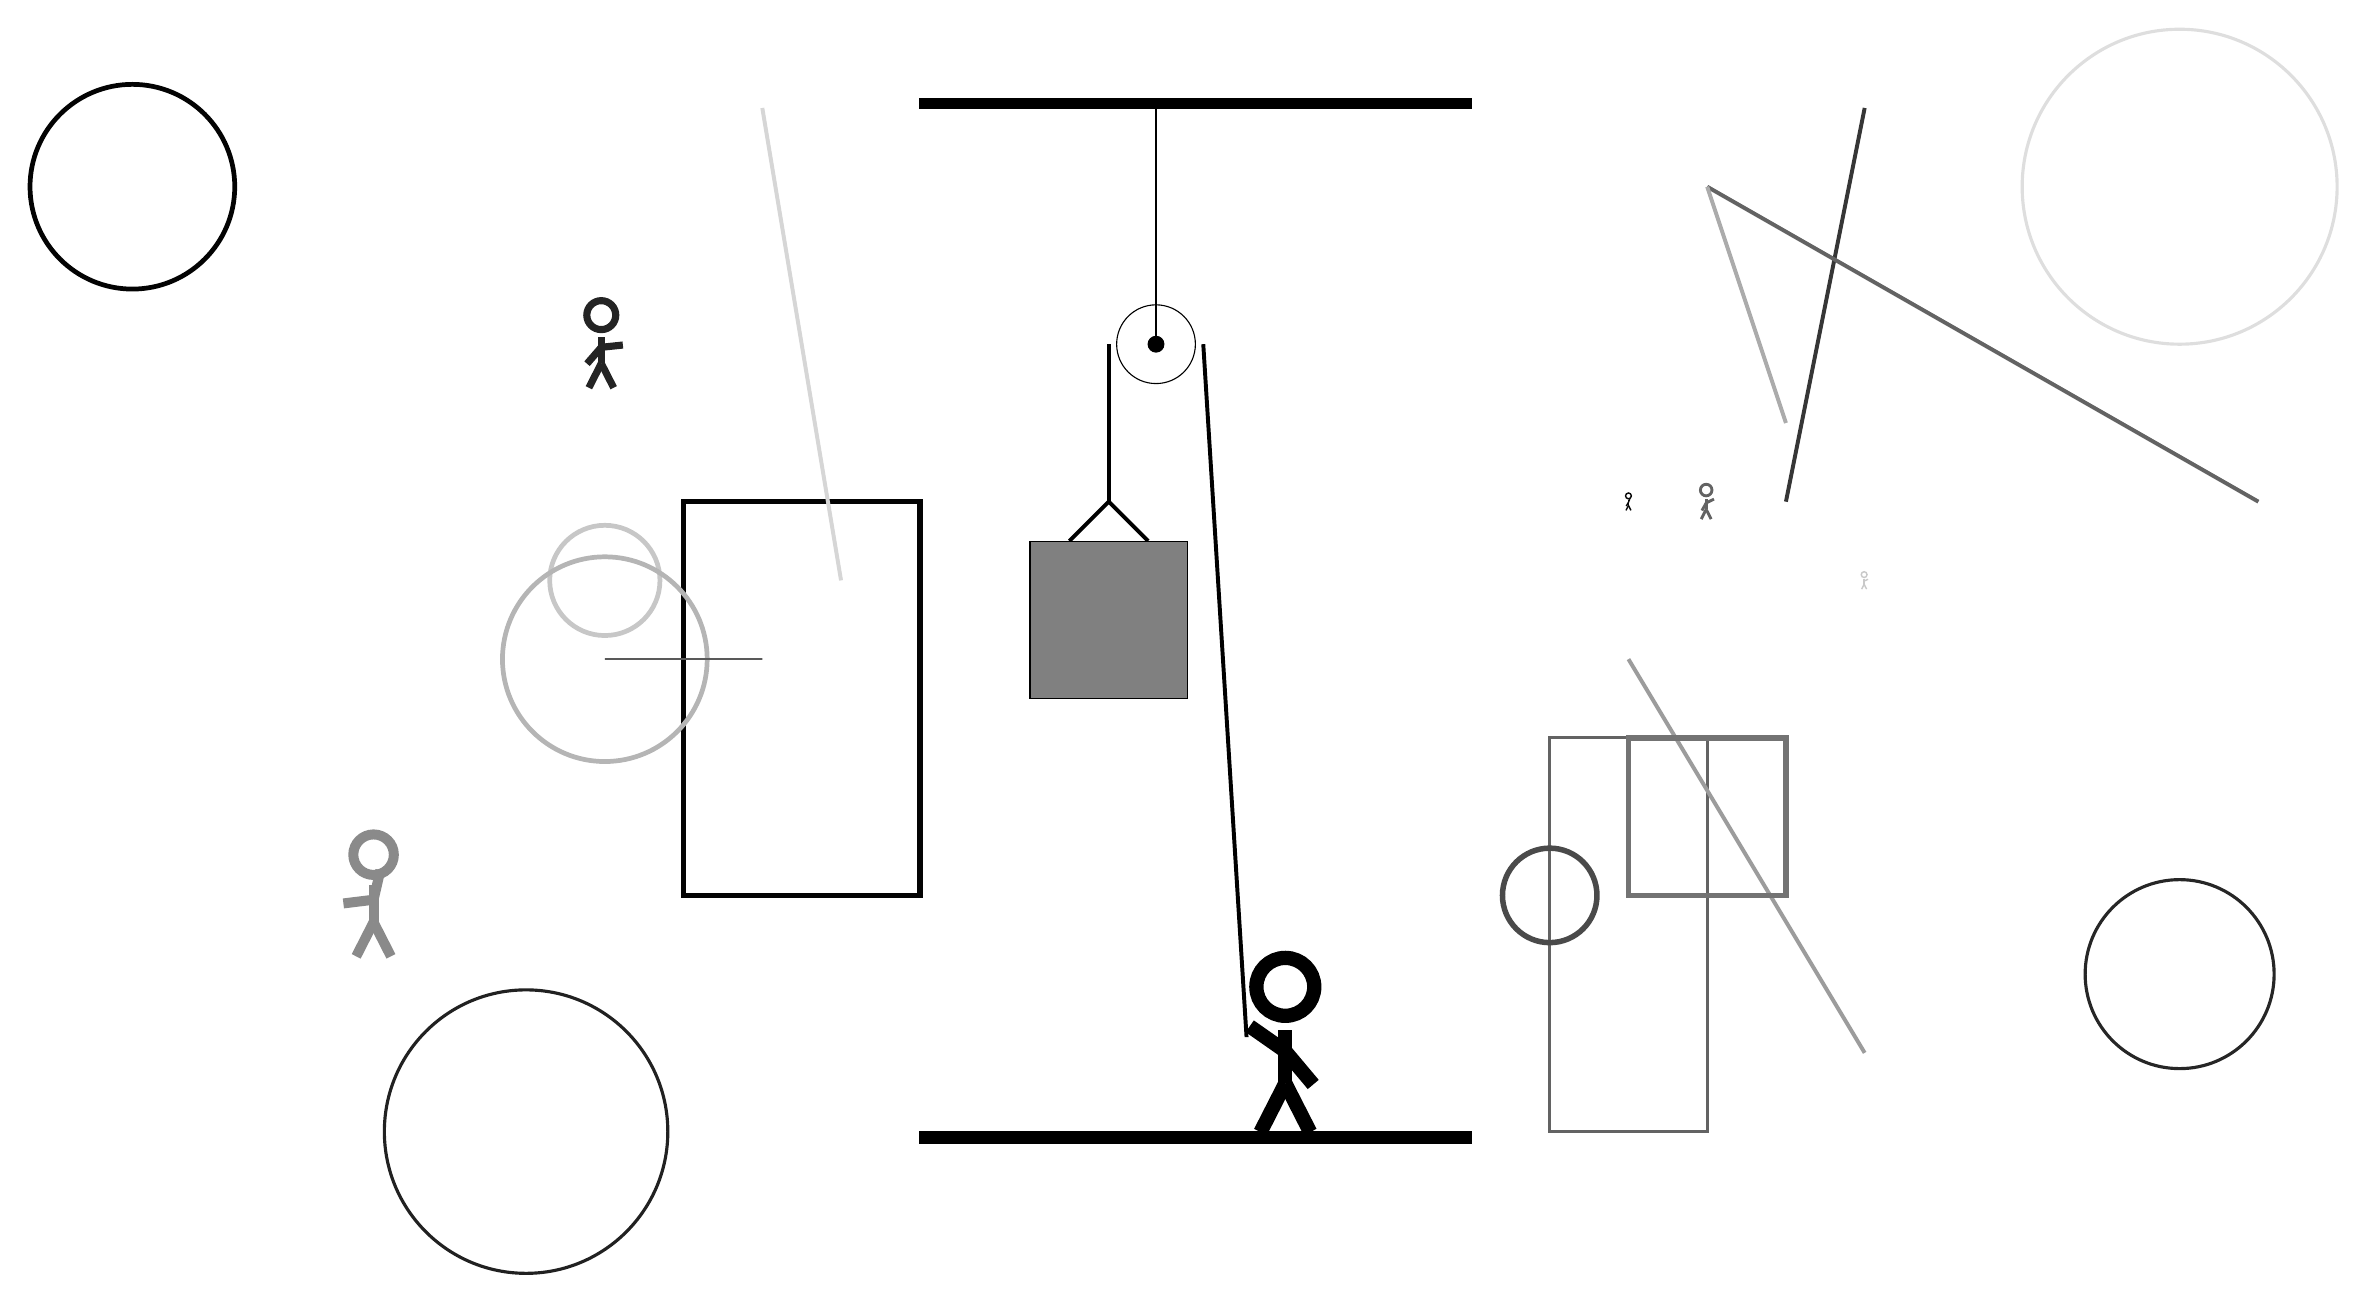
\begin{tikzpicture}
		%%%%% START %%%%%
		
		\draw[fill=black] (-2, 10) rectangle (5, 10.125);
		
		\draw (1, 7) circle (0.5);
		\draw[fill=black] (1, 7) circle (0.1);
		\draw (1, 10) -- (1, 7);
		
		\draw[line width=0.5mm] (-0.1, 4.5) -- (0.4, 5.0) -- (0.9, 4.5);
		\draw[fill=black!50] (-0.6, 4.5) rectangle (1.4, 2.5);
		
		\draw[line width=0.5mm] (0.4, 7) -- (0.4, 5.0);
		\centerarc[line width=0.5mm](1, 7)(0:180:0.6);
		\draw[line width=0.5mm](1.6, 7) -- (2.15, -1.8);
		
		\node at (2.6, -1.9) {\Strichmaxerl[10][-35][-50]};
		
		\draw [line width=0.6mm, color=black!22](-6, 4) circle (0.7);
		
		\draw [line width=0.7mm, color=black!39](-3, 5) circle (0.0);
		\draw [line width=0.4mm, color=black!85](14, -1) circle (1.2);
		\draw[line width=0.7mm, color=black!99] (-2, 5) rectangle (-5, 0);
		
		\draw[line width=0.4mm, color=black!61] (6, 2) rectangle (8, -3);
		\draw [line width=0.4mm, color=black!87](-7, -3) circle (1.8);
		\node[line width=0.3mm, color=black!21] at (10, 4) {\Strichmaxerl[1][85][24]};
		
		\draw[line width=0.5mm, color=black!16](-4, 10) -- (-3, 4);
		\draw [line width=0.6mm, color=black!29](-6, 3) circle (1.3);
		
		\draw[line width=0.5mm, color=black!39](7, 3) -- (10, -2);
		
		\node[line width=0.4mm, color=black!97] at (7, 5) {\Strichmaxerl[1][60][69]};
		\node[line width=0.6mm, color=black!86] at (-6, 7) {\Strichmaxerl[5][49][6]};
		\draw [line width=0.7mm, color=black!71](6, 0) circle (0.6);
		
		\draw[line width=0.7mm, color=black!55] (7, 2) rectangle (9, 0);
		\draw[line width=0.5mm, color=black!79](10, 10) -- (9, 5);
		\draw[line width=0.5mm, color=black!61](8, 9) -- (15, 5);
		
		\draw [line width=0.2mm, color=black!53](10, 2) circle (0.0);
		\node[line width=0.5mm, color=black!61] at (8, 5) {\Strichmaxerl[2][61][26]};
		\node[line width=0.3mm, color=black!46] at (-9, 0) {\Strichmaxerl[7][7][77]};
		
		\draw [line width=0.6mm, color=black!99](-12, 9) circle (1.3);
		\draw [line width=0.4mm, color=black!13](14, 9) circle (2.0);
		
		\draw[line width=0.2mm, color=black!65] (-4, 3) rectangle (-6, 3);
		\draw[line width=0.5mm, color=black!33](9, 6) -- (8, 9);
		
		\draw[fill=black] (-2, -3) rectangle (5, -3.15);
		
		%%%%% END %%%%%
	\end{tikzpicture}
\end{document}